\section{GPU-enabled parallel Schr\"odinger simulations}
\label{sec:3D Stirap parallel Schr\"odinger simulations}

Here I will introduce the problem of atomic transport in cold atomic systems, present the resulting model system, and give all the essential physics. Controlling the centre-of-mass movement of atoms has recently become a popular topic of investigation \cite{AO:SAP_REVIEW_2016}. One family of techniques that aim to solve this are those of \textit{spatial adiabatic passage} (SAP). In the following section I will describe the motivation, physical system, and the numerical implementation for the solution of the problem of transporting a single atom among three trapping potential wells. The fully three-dimensional numerical solution of this problem will then be provided using GPU computing methods, and the results discussed for both the physical and computing aspects.

For performance metrics, I will discuss the use of a GPU-enabled Schr\"odinger equation integrator developed by myself, based on and compared with the results to a multi-core MPI enabled version by T. Morgan and N. Crowley. The solution of the Schr\"odinger equation for a fully three-dimensional potential, will demonstrate the effectiveness and improved performance compared to standard HPC methods.

\subsection{Spatial adiabatic passage}
Controlling the internal degrees of freedom of atoms is well understood and many optical techniques exist. External degrees of freedom have, however, only recently become interesting due to the advancements in atom trapping, and techniques for controlling the centre of mass state of a single atom are still in development. One promising group of techniques for the generation of spatial superposition states or high fidelity transfer relies on ideas from spatial adiabatic passage \cite{AO:SAP_REVIEW_2016}, which are analogous to STIRAP in optical systems~\cite{AO:Bergmann_jcp_2015}. These techniques are highly robust against variation in the system parameters \cite{Eckert:04}, but suffer from being slow due to the adiabatic requirement. The use of this technique has recently been experimentally demonstrated in Lieb lattices \cite{AO:Taie_oist_2016}, and many other accessible systems have been proposed \cite{Eckert:06,Morgan:11,Kohler:13}.

To describe this method, I will first consider the case of a two-state system, which can be realised using two separated harmonic potential traps, with groundstates $| L \rangle$ and $| R \rangle$. A reduction of the distance between the traps will increase the coupling, and hence tunneling rate, between them. This is modeled with the two-level Hamiltonian as
\begin{equation}
    H = -\frac{\hbar}{2}
    \begin{pmatrix}
        0 & J_{LR} \\
        J_{RL} & \Delta
    \end{pmatrix}
\end{equation}
where $J_{LR} = J_{RL}$ are the couplings between states, and $-\Delta$ is the detuning of state $| R \rangle$, relative to $| L \rangle$. Assuming an atom initially localised in $| L \rangle$, and with an increase in coupling strength between the levels, the localised atom will tunnel from $| L \rangle$ to $| R \rangle $. However, this processes is difficult to control, as Rabi oscillations introduce an explicit time-dependence as
\begin{subequations}
\begin{align}
    |c_L(t)|^2 &\propto \sin^2 \frac{\omega t}{2} ,\\
    |c_R(t)|^2 &\propto 1 - |c_L(t)|^2,
\end{align}
\end{subequations}
where $|c_{L,R}(t)|^2$ are the populations of the respective states. This time dependence causes the atomic population to continuously transfer between both traps. It will therefore require precise timing and control to ensure a full, robust transfer of population. From this we see that a double-well potential is a difficult system in which to realise coherent control, though methods such as rapid adiabatic passage (RAP) exist and can allow for this~\cite{AO:Vitanov_arpc_2001}. A more robust method, using three adjacent harmonic traps and the aforementioned matter-wave SAP process, can improve upon the standard double-well system. For this SAP technique, we model the trapping potentials arranged in a single line and coupled with their nearest neighbour solely. For three such potentials, $L,M,R$, on resonance, the system can be described by the Hamiltonian
\begin{equation}\label{eqn:sap_ham}
    H = -\frac{\hbar}{2}
    \begin{pmatrix}
        0 & J_{LM} & 0 \\
        J_{LM} & 0 & J_{MR} \\
        0 & J_{MR} & 0
    \end{pmatrix},
\end{equation}
where $J_{LM},~J_{MR}$ describe the left-middle and middle-right couplings respectively. Diagonalising this Hamiltonian gives three distinctive eigenstates,

\begin{subequations}
\begin{align}
| \pm \rangle = \frac{J_1 |L\rangle \pm \sqrt{J_1^2 + J_2^2}|M\rangle + J_2 |R\rangle  }{\sqrt{2(J_1^2 + J_2^2)}} \\
| D \rangle = \frac{J_2 |L\rangle }{\sqrt{J_1^2 + J_2^2}} - \frac{J_1 |R\rangle}{\sqrt{J_1^2 + J_2^2}}
\end{align}
\end{subequations}
with respective eigenvalues $E_{\pm} = \pm {\sqrt{J_1^2 + J_2^2}}$, $E_D = 0$.
Here, only one eigenstate is of interest. For the zero-valued eigenstate of this Hamiltonian, $|D \rangle$, known as the \textit{dark state}, the dependence on the middle potential vanishes. The state can be written as
\begin{equation}
 | D \rangle = \cos\ \Theta| L \rangle - \sin \Theta | R \rangle,
\end{equation}
where $\tan \Theta=J_{LM}/J_{MR}$ is the mixing angle, following directly from the trigonometric identities $\cos (\arctan (x)) = 1/\sqrt{1+x^2},\sin (\arctan (x)) = x/\sqrt{1+x^2}$. From the adiabatic theorem of quantum mechanics, it is known that if a system has its Hamiltonian perturbed slowly enough, then we can follow its evolution ensuring that it always remains in an eigenstate of the Hamiltonian. By preparing the system in state $| L \rangle$, and varying $\Theta$ slowly, we can shift the population from the leftmost harmonic potential to the rightmost, without populating the center. Coupling profiles that have been investigating for this have been both Gaussian \cite{AO:Bergmann_jcp_2015} and sinusoidal, with a respective delay of the second pulse to allow for a smooth variation of $\Theta$. This can be performed by modulating the pump frequencies by a smoothly varying background envelope $p$ as \cite{AO:Fewell_ausjp_1997}
\begin{subequations}
\begin{align}
    \Omega_{LM}(t) = \Omega_0 p(t-\tau) \\
    \Omega_{MR}(t) = \Omega_0 p(t),
\end{align}
\end{subequations}

Varying the couplings between trapping potentials, and hence controlling this mixing angle, can be achieved by either lowering the barrier height of adjacent potentials, or decreasing the distance between them. Here, I will discuss the use of varying the spatial separation of the traps. To ensure full transfer from $|L \rangle$ to $| R \rangle$, the mixing angle must vary smoothly from $\Theta = 0 \rightarrow \pi/2$. Given the properties of $\arctan$, this can be achieved by applying the same spatial variation between $|M \rangle$ and $| R\rangle$, as between $|L \rangle$ and $| M\rangle$, with the latter pulse following a delay, $\tau$. A diagram of this is given by Fig.~\ref{fig:ch3_stirap}.


\begin{figure}
    \centering
    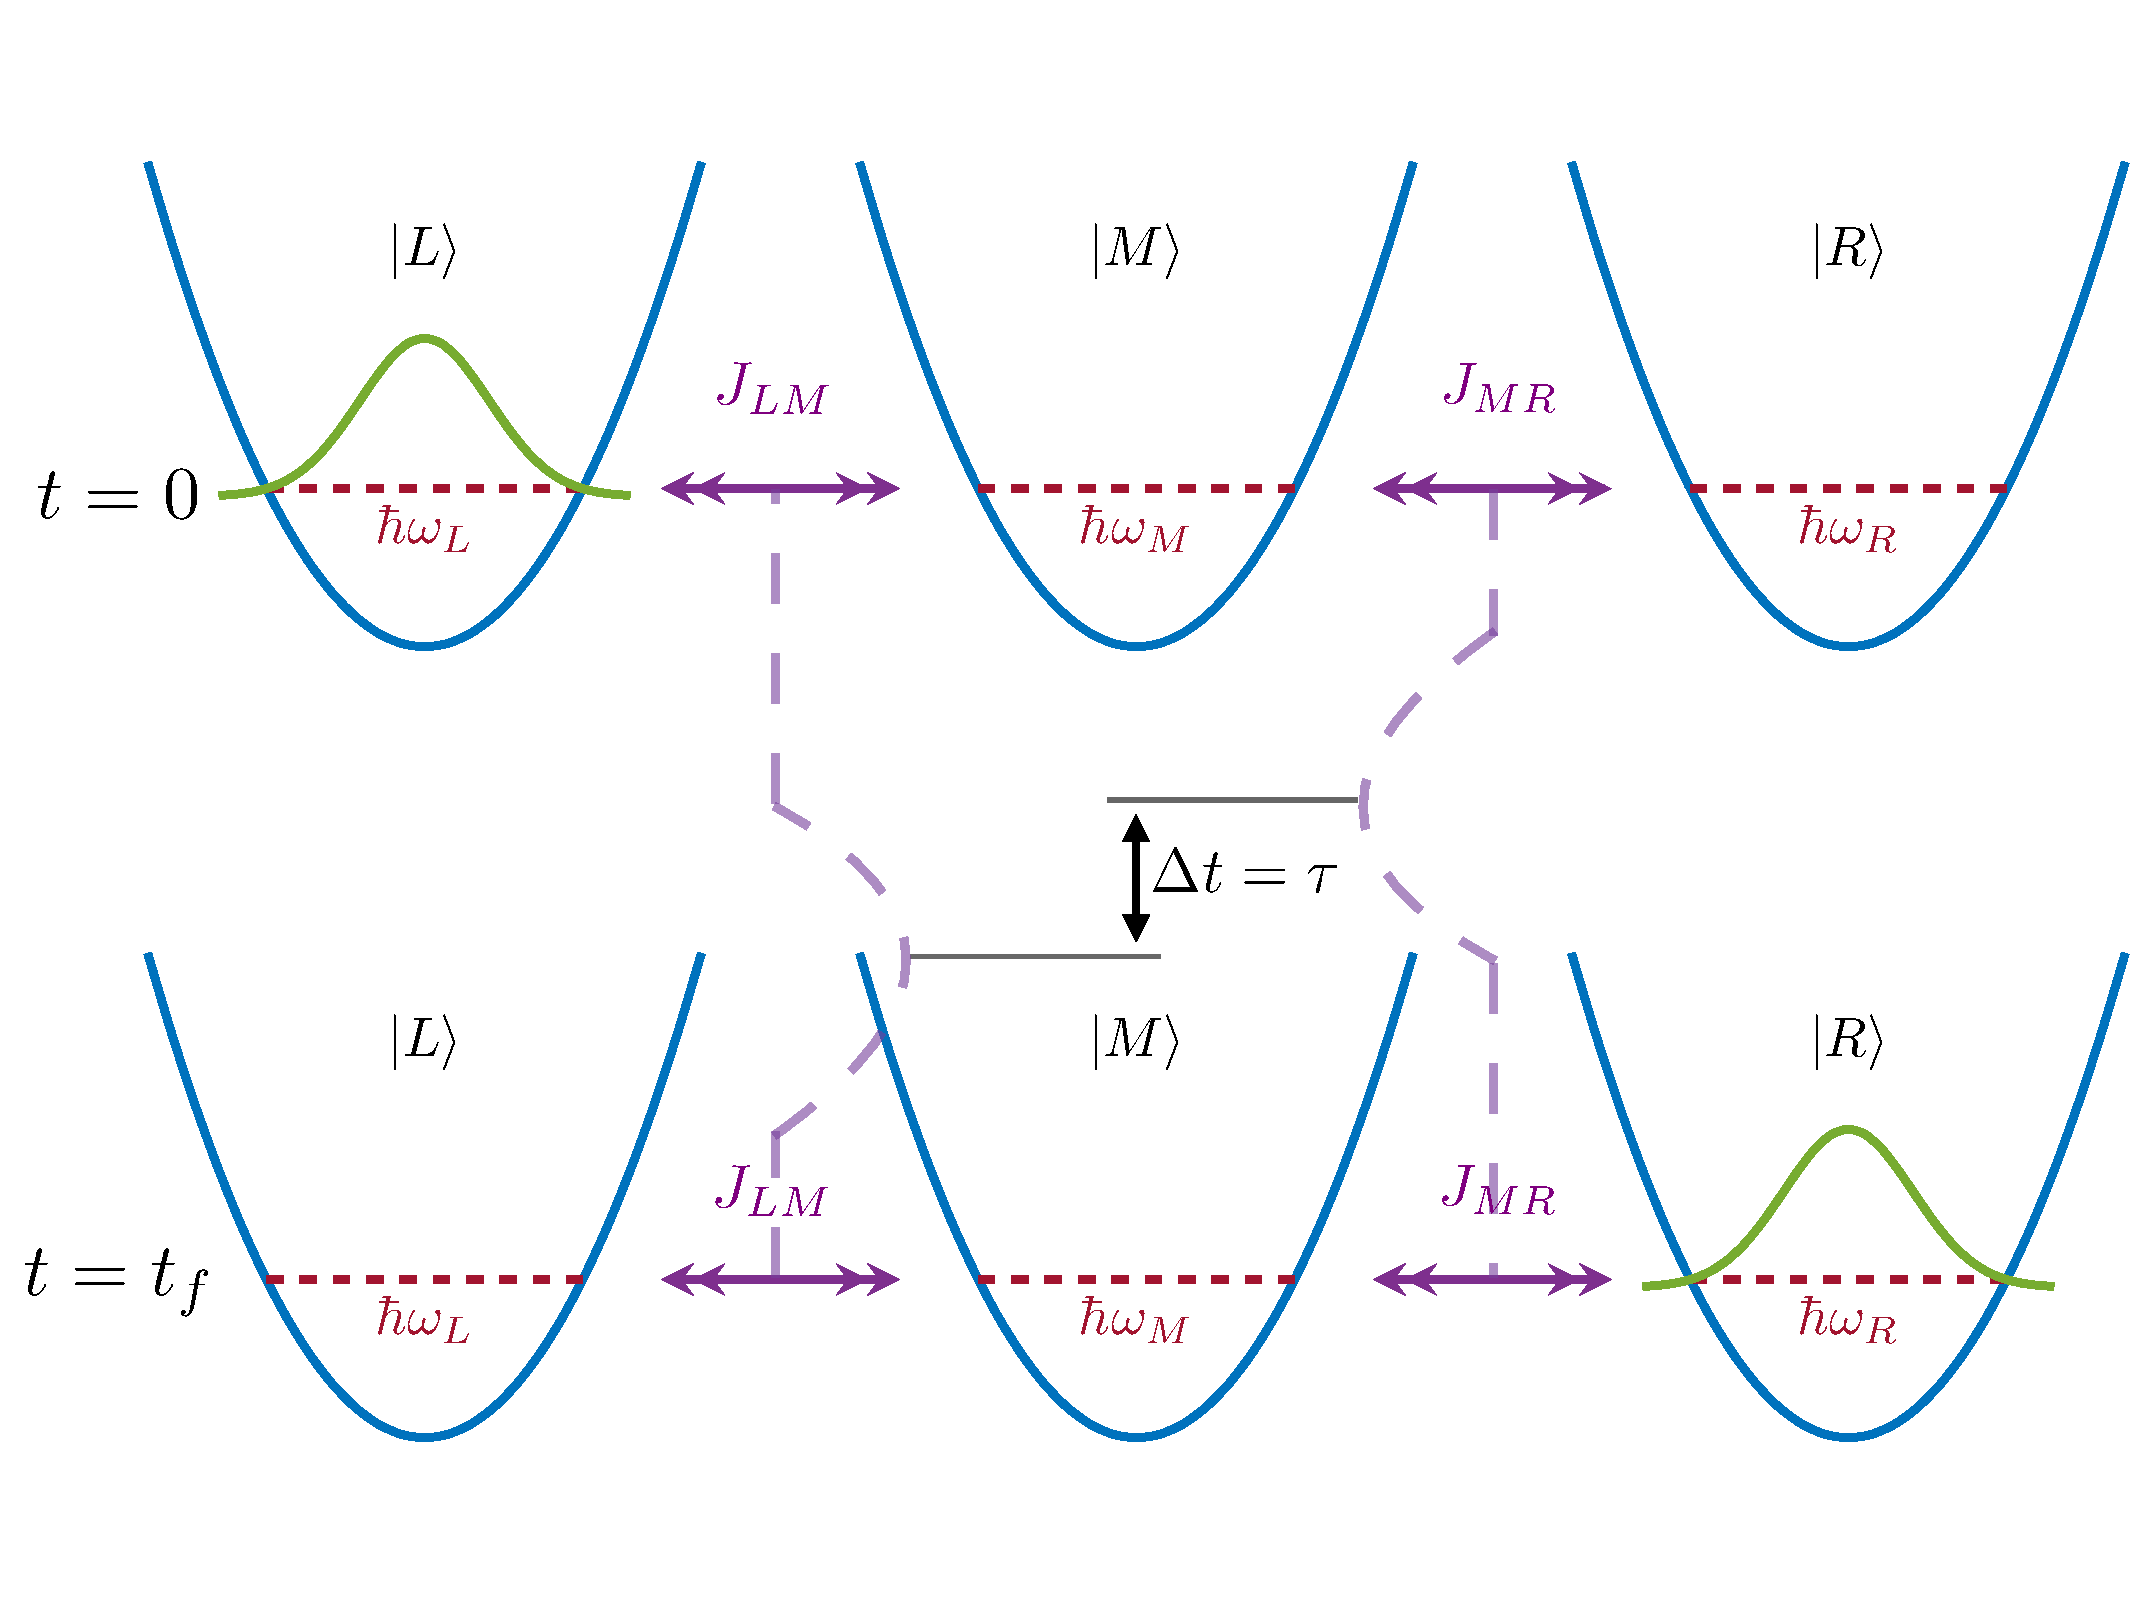
\includegraphics[width=0.65\textwidth]{./ch3_numerics/stirap_delay}
    \caption{Three trapping potential model for matter-wave SAP. The atom (green) is initially localised in the leftmost potential, $|L\rangle$, at $t=0$, with the couplings between adjacent traps controlled by varying the distance dependent parameters $\Omega_{LM} = J_{LM}$, $\Omega_{MR} = J_{MR}$. By varying the couplings between traps in the manner shown, with $\Omega_{MR}$ increasing initially, followed by $\Omega_{LM}$ after a delay $\tau$, the atom is transfered completely from $|L\rangle$ to $| R \rangle$.}
    \label{fig:ch3_stirap}
\end{figure}

%With the rate of transfer between trapping potentials controlled by the couplings between potentials, any adjustment of the spatial separation between traps will adjust the tunneling rate, and hence couplings, as shown by Fig.~\ref{fig:ch3_stirap}.
Typically, any method to adjust the couplings would be performed with time-dependent potentials. However, a static potential variant can be considered using parallel atomic waveguides, where the separation varies as a function of distance along the parallel axis. If we consider an atom that travels along such a waveguide, the coupling and hence tunneling rates seen by the atom in the waveguide are altered as the atom propagates. Such work has been discussed and considered in a realistic system for two spatial dimensions \cite{OSullivan:10}. Although a two dimensional model is effective at describing much of the relevant dynamics, the lack of a third dimension ensures the effects stemming from dispersion, curvature of the waveguides and the absence of any such eigenstates along this dimension reduce the realism of such a model.

\subsection{Atom-chip model}

As discussed previously, to fully understand the dynamics of in appropriately shaped waveguide systems we must investigate the fully three-dimensional model. One method of creating the required potential landscape is through the use of atom-chips \cite{AO:Bartenstein_ieee_2000,AO:Folman_prl_2000}. These systems consist of micro-fabricated current-carrying wires, and can be used to create a variety of trapping potential shapes for controlled guidance of atomic centre-of-mass \cite{AO:Denschlag_prl_1999}. The currents produce a magnetic field around individual wires, each of which has a minima at the wire core. Assuming the wire thickness to be negligible, this magnetic field at position $\mathbf{r}$ can be calculated using the Biot--Savart law
\begin{equation}
    \mathbf{B}(\mathbf{r}) = \frac{\mu_0}{4\pi}\oint I \frac{\text{d}\mathbf{l}\times \hat{\mathbf{r}}^{'}}{|\mathbf{r^{'}}|^2},
\end{equation}
where $I$ is the current through the wire, $\mu_0$ is the vacuum permeability, $\text{d}\mathbf{l}$ is the differential wire length, and $\hat{\mathbf{r}}^{'}$ is the unit vector along $\mathbf{r^{'}} = \mathbf{r} - \mathbf{l}$. For the resulting field to trap atoms the minima must be raised to a position above the wire surface. This can be done using an orthogonally applied bias field, ${B}_b$, which raises the minima to a height of
\begin{equation}
    \mathbf{r}_0 = \frac{\mu_0 I}{2\pi {B}_b},
\end{equation}
above the surface. Though, an issue still remains with the presence of the magnetic minima. If the field drops to zero at the centre of the trap, the atoms can be lost due to Majorana spin flips~\cite{AO:Brink_pra_2006}. This can be prevented with the application of an additional field, ${B}_{p}$, parallel to the wire direction, lifting the degeneracy of the atomic states, and ensuring they remain trapped. Spatial and temporal adjustments of the potentials are possible, with a fine degree of control, either during the production process, or by using time-dependent currents. These have been studied extensively in recent years for highly controllable trapping potentials \cite{AO:Yun_optexp_2006,AO:Gallego_optlett_2009}, and as atomic manipulators \cite{AO:Bensky_qip_2011}, to mention but a few.

For this work, the system was modeled as three adjacent wires on the atom-chip surface. As the magnetic minima travel along the length of a atom-chip surface in $z$, we assume that the magnetic fields can be considered as adjacent trapping potentials in the $x-y$ plane. The direction of propagation is then along $z$, where the presence of an additional harmonic oscillator potential, $V_z$, is applied to impart motion to the atom, which begins at the $z=0$ position of the atom-chip. This potential also conveniently guarantees that the wavefunction refocuses after the transition at the opposite side of the atom-chip. A schematic of the atom-chip device and the respective potentials is given by Fig.~\ref{fig:schematic_atom-chip}.

\begin{figure}[tb]
    \centering
  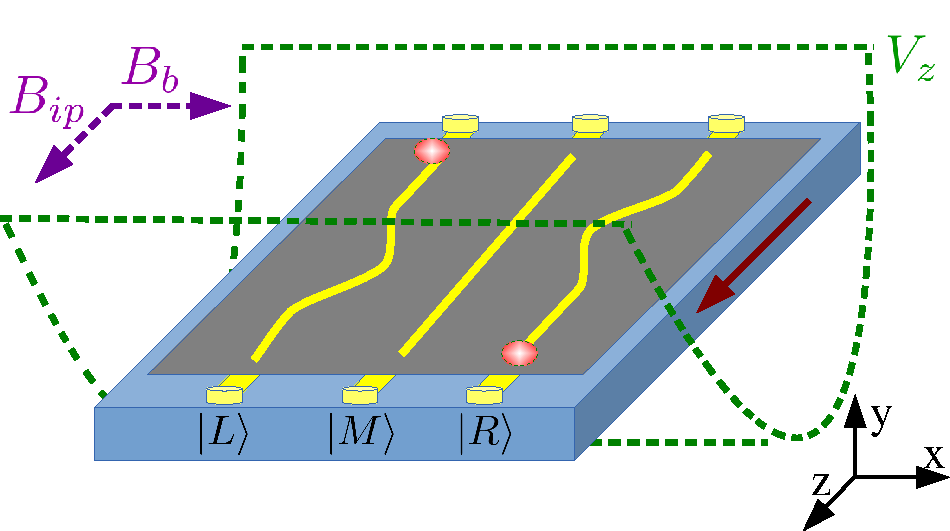
\includegraphics[width=0.45\textwidth]{ch3_numerics/MWSTIRAP/Schematic3}
  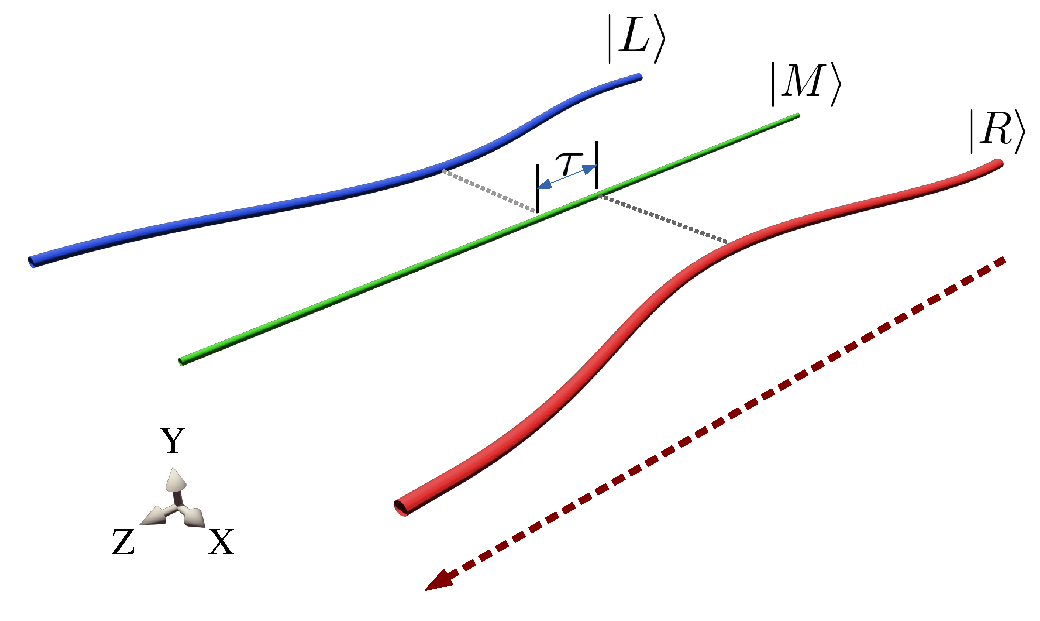
\includegraphics[width=0.45\textwidth]{ch3_numerics/MWSTIRAP/3dpot_schem}
  \caption{Schematic of the atom-chip and the resulting potentials. Copyright PRA...}
  \label{fig:schematic_atom-chip}
\end{figure}

The initial state is created by localising the atom with the help of a barrier at one end of the potential, and on the left using an additional barrier potential. After finding the the groundstate, the barriers were removed, and the atom was allowed to propagate along the length of the waveguide. The populations in each waveguide $|c_{X}|^2$ were tracked at each step of the process as
\begin{equation}
    |c_X|^2 = \int\limits_{\mathcal{V}_X} d\mathbf{r}  \Psi^{*} \Psi
\end{equation}
where $\mathcal{V}_X$ is the volume encompassing each waveguide $X \in \{L,M,R\}$, and $| \Psi \rangle$ is the state of the system.
The final populations were taken as the atom approached the end of the harmonic oscillator along $z$. The fidelity of the process could then be calculated by comparing the initial populations in $| L \rangle$ and final ones in $|R \rangle$, as well as any ones left in $| M \rangle$.

Given that fully three-dimensional simulations of the Schr\"odinger equation are numerically expensive, the use of GPU computing methods were ideal for accelerating the simulation \cite{Num:Bauke_cpc_2011}. At that time, as far as we had been aware, no other work using GPU computing to solve a three dimensional Schr\"odinger equation had been presented. I will now discuss the resulting data and metadata of the simulations.

\subsection{3D Simulations}
\label{sec:Results}

Simulations of the proposed system assumed a single $^{6}$Li atom localised in the left waveguide. Its transversal wavefunction was determined numerically, with the assumption of a longitudinal Gaussian profile of similar width. The atom was then allowed to propagate along the waveguide potential ($z$).

As the shift in magnetic moment of the atoms is given by $\Delta E = -\mu\cdot\mathbf{B}$, for regions with a larger magnetic field the atom will experience a greater energy shift, and thus the assumption of all traps in resonance is no longer valid. The simulations showed that the addition of the magnetic fields stemming from the different wires at the center of the atom-chip leads to the central potential moving out of resonance with the outer two. This required adjusting the current in the central wire, such that the magnetic minima were in resonance within the tunneling region. The resulting potentials for non-optimal (left) and optimal (middle) currents are shown in Fig.~\ref{fig:equaloptcurrent}, which also depicts a three dimensional isosurface of the potential minima along the chip surface (right).

\begin{figure}[tb]
    \centering
  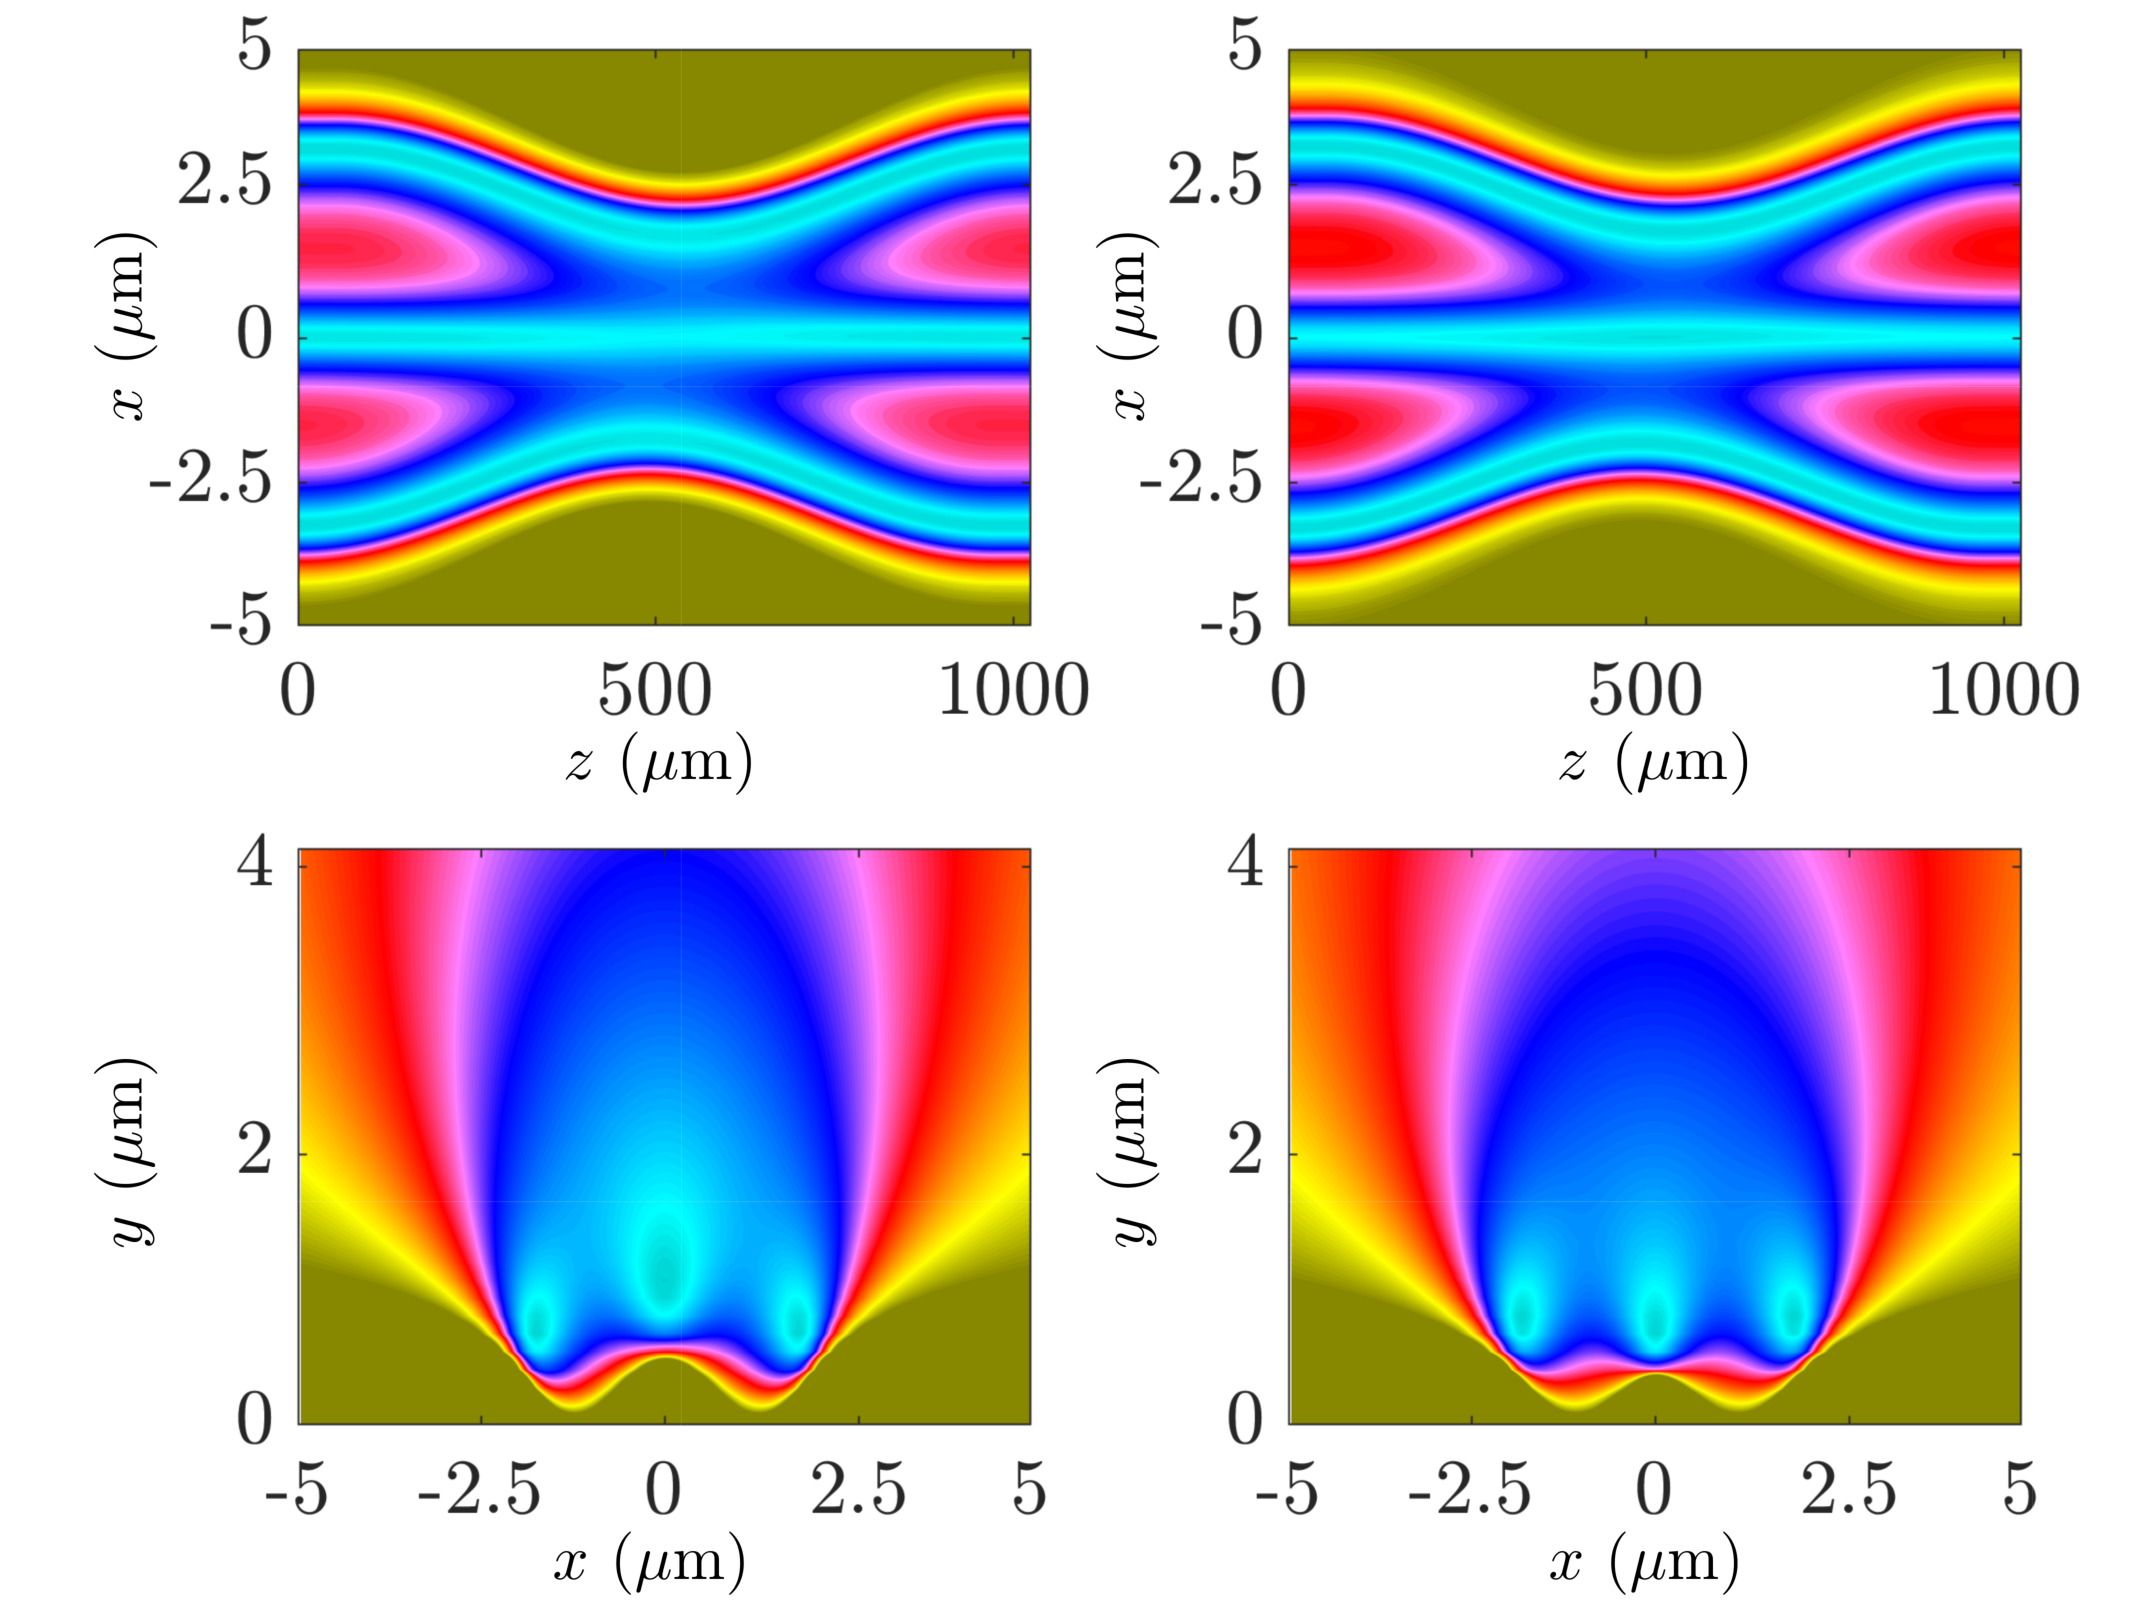
\includegraphics[width=0.55\textwidth]{ch3_numerics/MWSTIRAP/potentials2.pdf}
  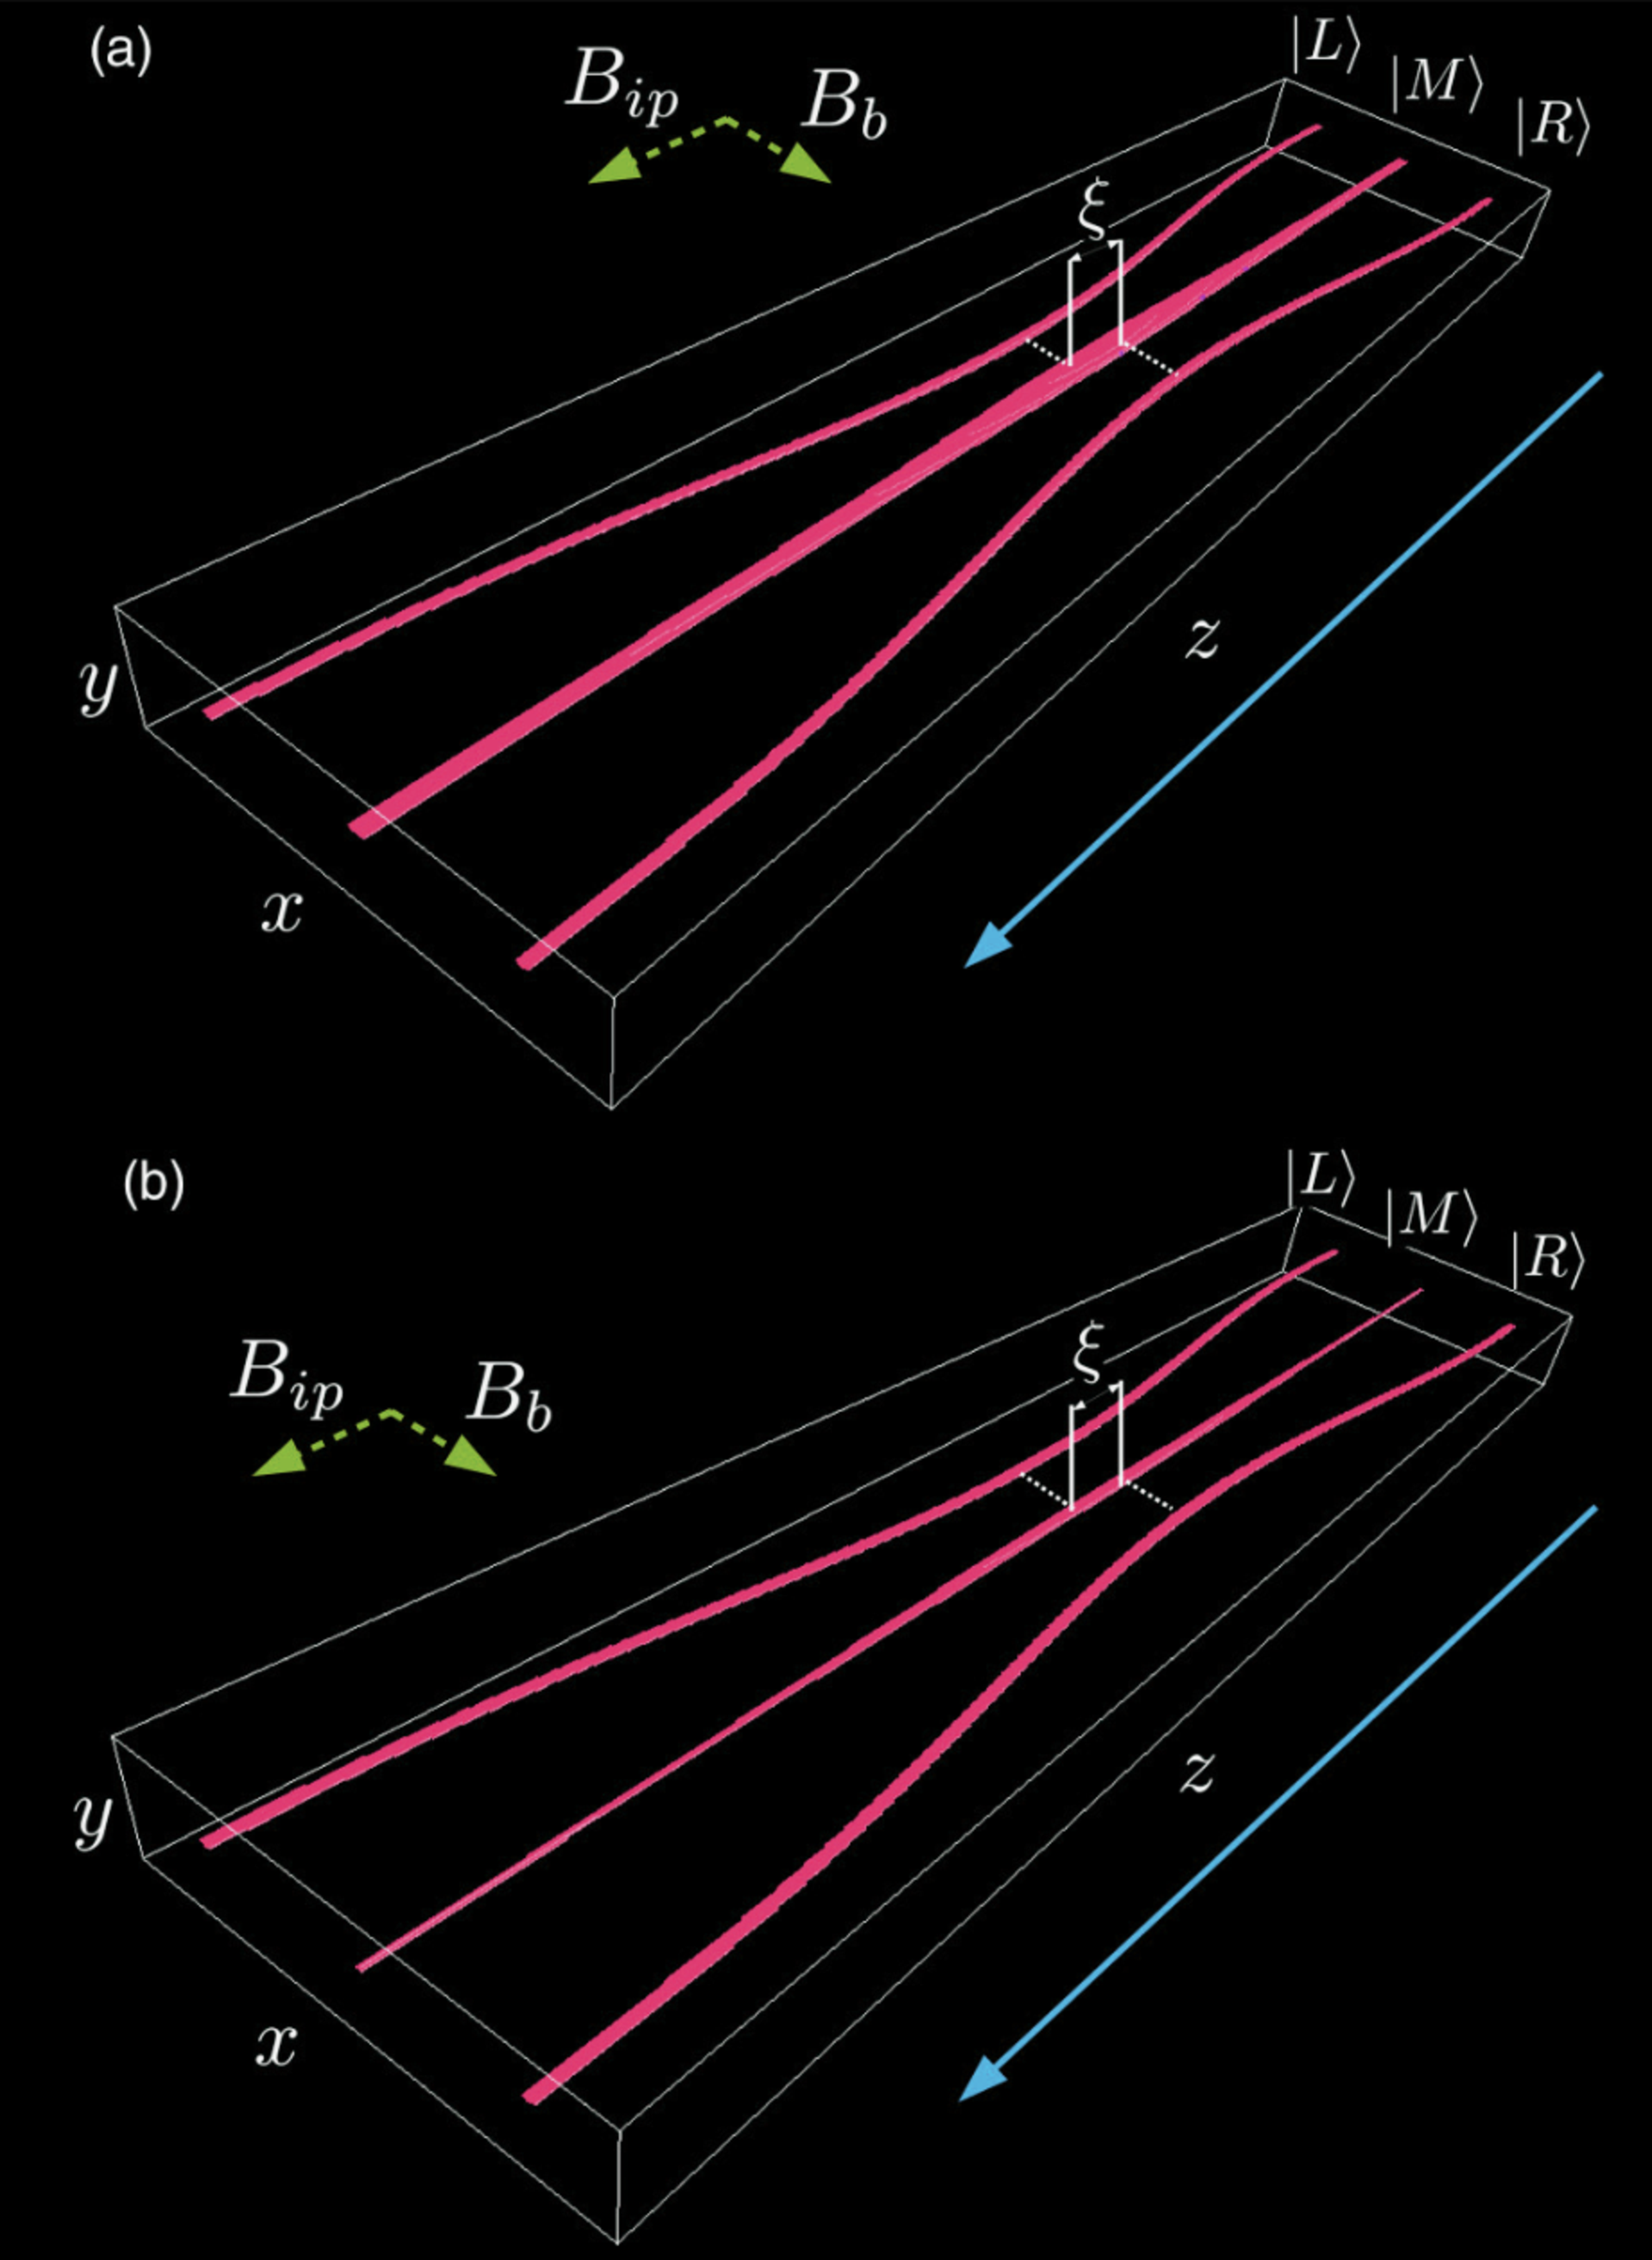
\includegraphics[width=0.3\textwidth]{ch3_numerics/MWSTIRAP/3dpot.pdf}
  \caption{(Left) Two dimensional slices through the potential centre along $x-z$ (top) and tunneling region in $x-y$ (bottom). The out of resonance middle trapping potential can be seen where all three currents are the same. (Middle) Optimised currents which allow the same field value in the tunneling region ensure that the potentials are in resonance with the other potentials. (Right) 3D isosurface plots of the numerically calculated magnetic minima potentials showing the out of resonance (top) and optimal (bottom) fields.}
  \label{fig:equaloptcurrent}
\end{figure}

The populations for both the direct tunneling case, and the matter-wave SAP processes are shown in Fig.~\ref{fig:mwsVsDT}. The direct tunneling case can be seen to show Rabi-type oscillations between the waveguides, while the matter-wave SAP process shows a much cleaner transfer, and only a minor occupation of the central potential. The dependence of the transfer probability on the current in the central wire is shown in Fig.~\ref{fig:DIRVSMWSTIRAP}.


\begin{figure}[tb]
    \centering
  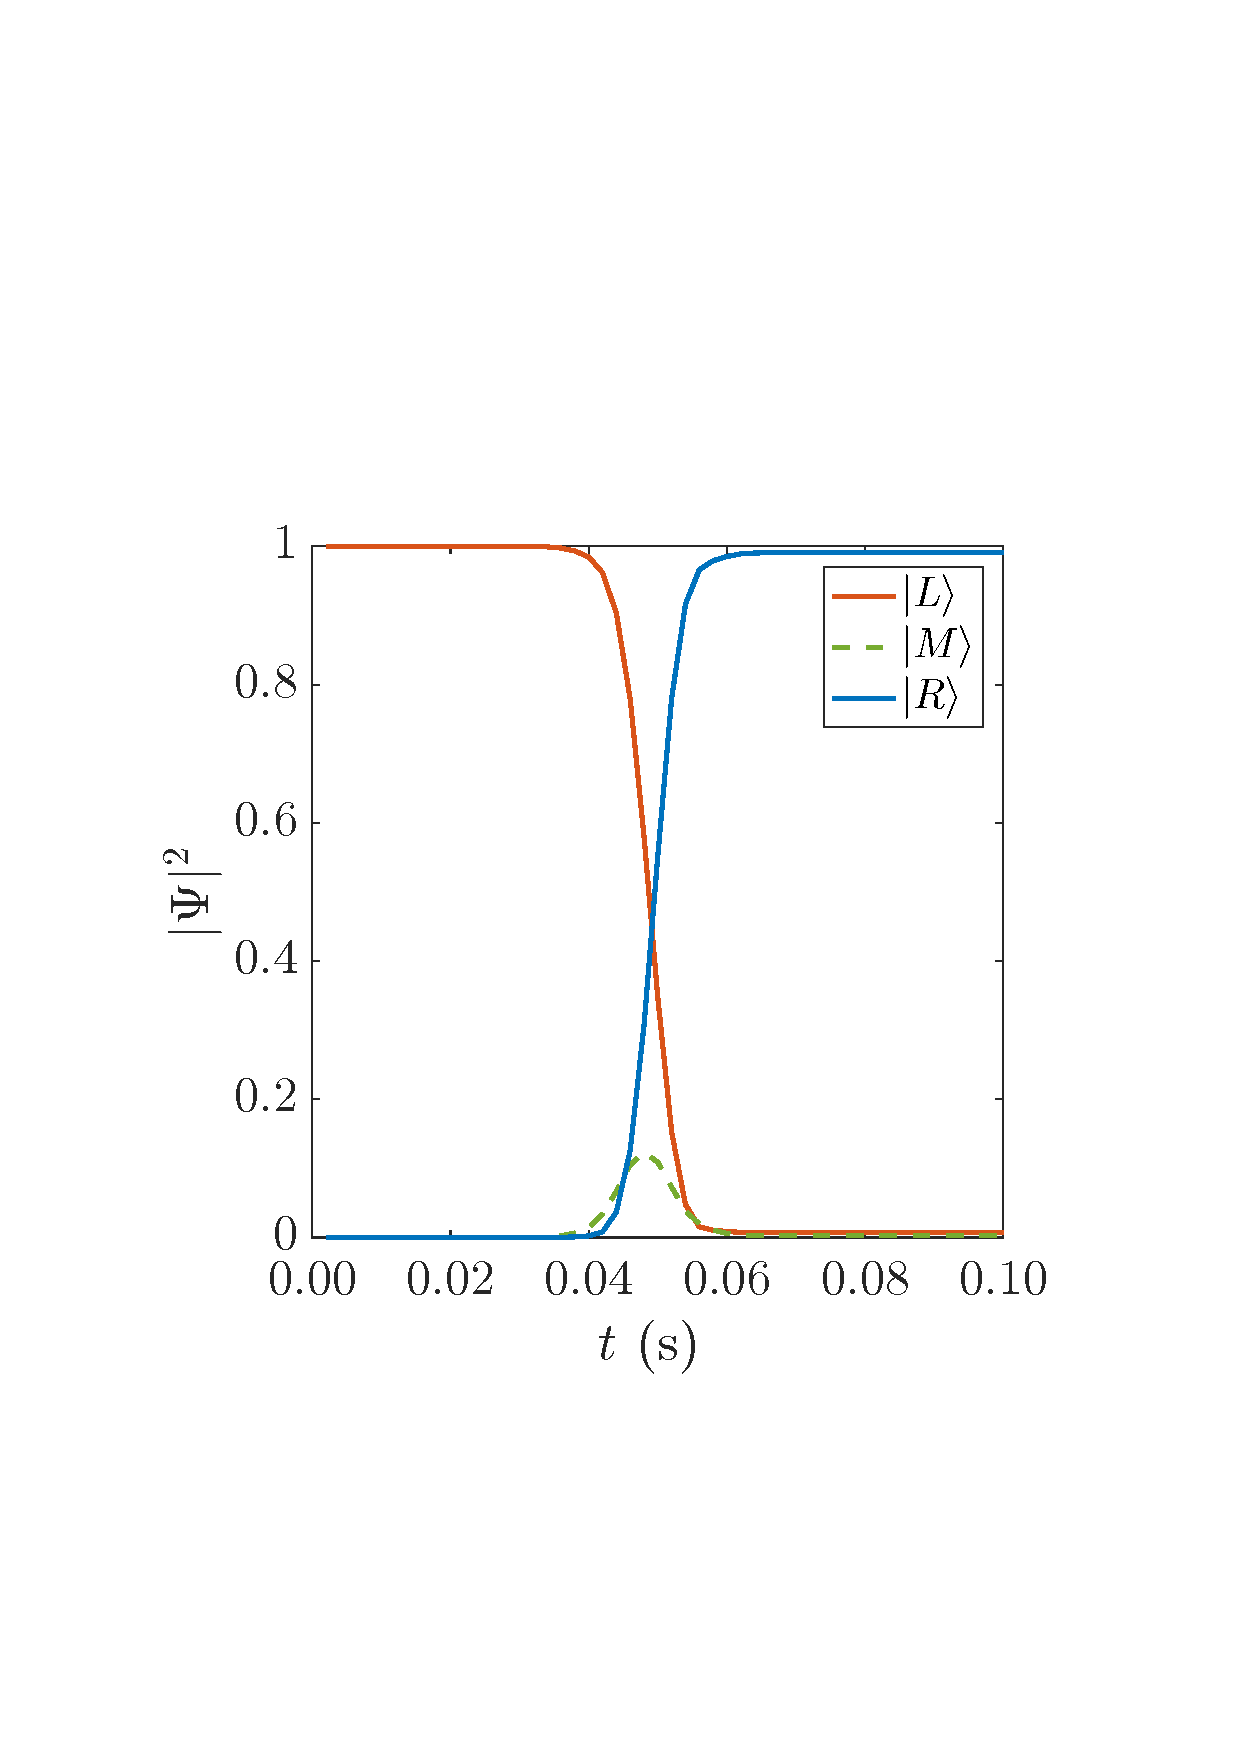
\includegraphics[width=0.47\textwidth,trim=2cm 5cm 2cm 5cm]{ch3_numerics/MWSTIRAP/STIRAP_CINT_POP.pdf}
  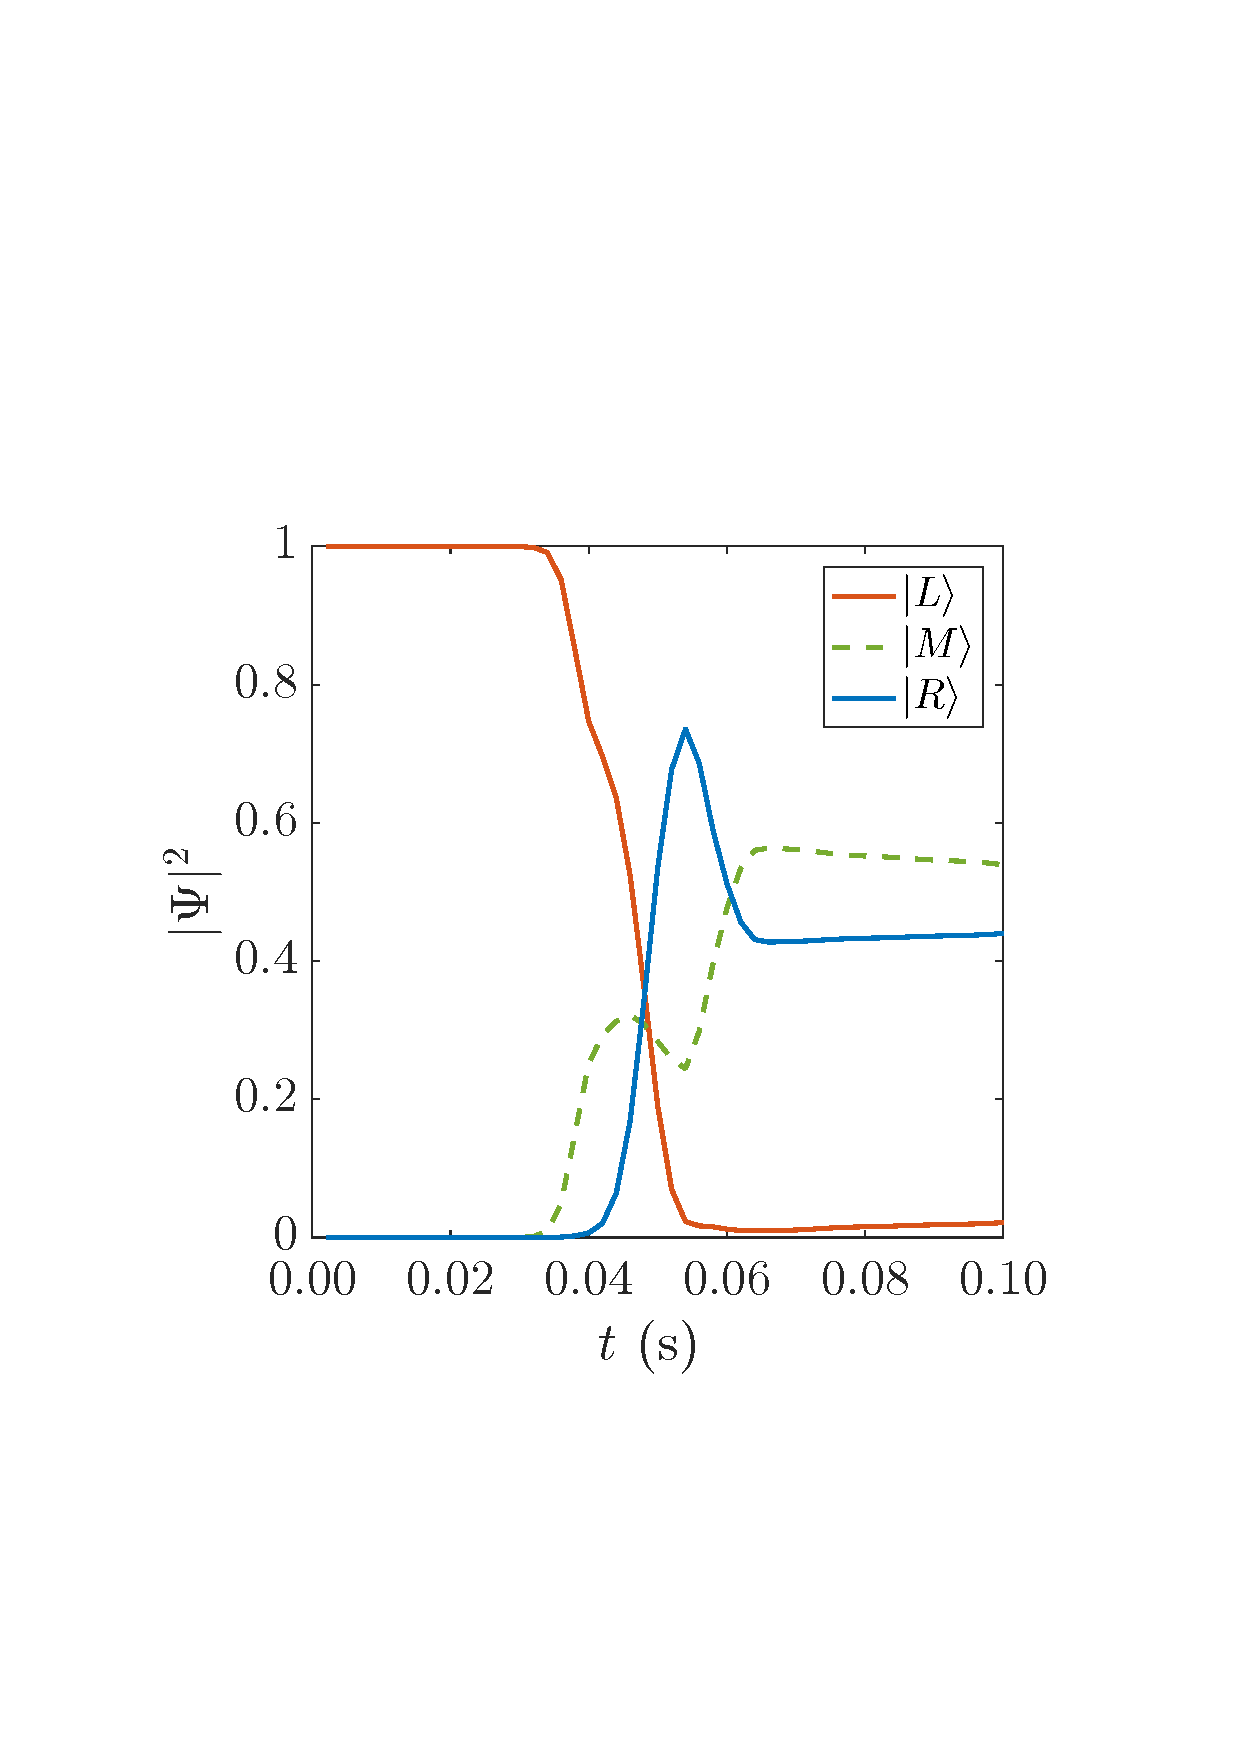
\includegraphics[width=0.47\textwidth,trim=2cm 5cm 2cm 5cm]{ch3_numerics/MWSTIRAP/STIRAP_INT_POP.pdf}
  \caption{Transfer fidelities for the three trapping potentials are given over time for both the matter-wave SAP process (left) and direct tunneling (right). Matter-wave SAP clearly shows greater population transfer in comparison with a direct tunneling approach.}
  \label{fig:mwsVsDT}
\end{figure}

\begin{figure}[tb]
    \centering
  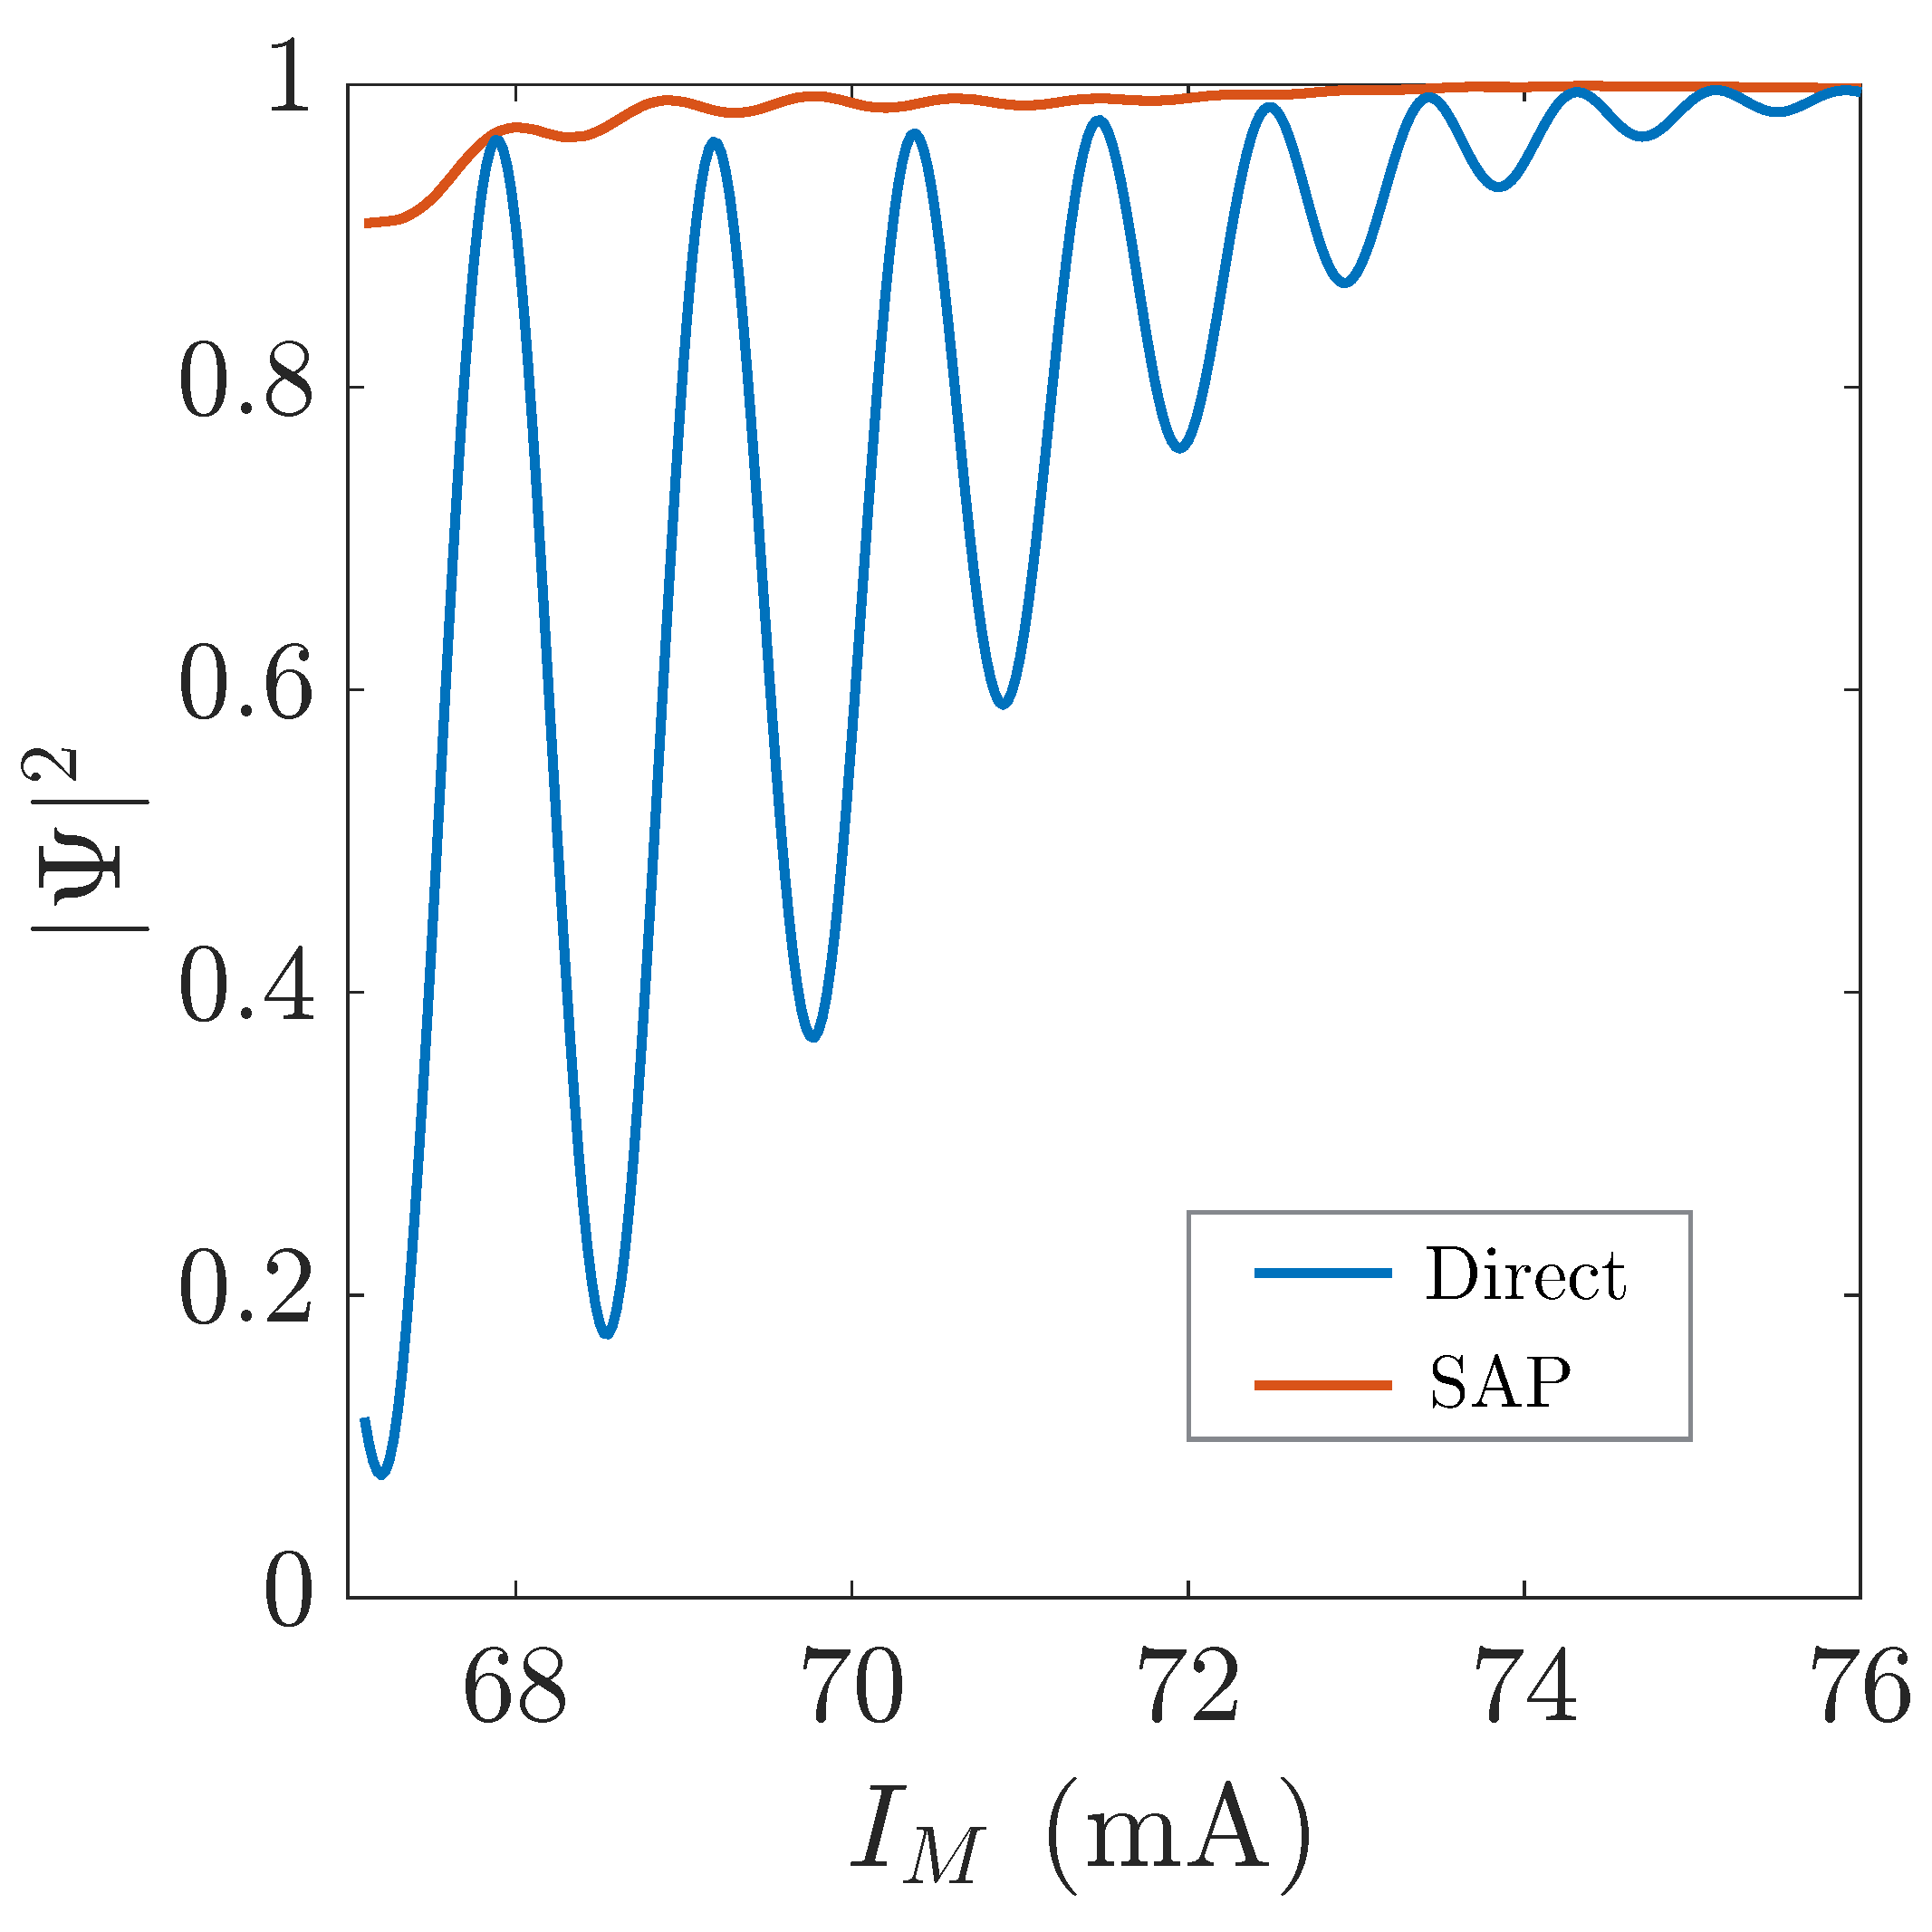
\includegraphics[width=0.45\textwidth]{ch3_numerics/MWSTIRAP/SAPvsDirect.pdf}
  \caption{The final state population versus middle wire current for direct tunneling and matter-wave SAP. The robustness of the SAP technique can be seen, and gives a large range of currents with population transfer fidelity $\approx 99 \%$. The oscillations in the direct tunneling regime are due to the time-dependent nature of the Rabi couplings.}
  \label{fig:DIRVSMWSTIRAP}
\end{figure}

%%

\subsection{GPU computing performance}
Given the large parameter space over which this system could be evaluated (e.g wire current, spatial separations, trap frequencies), many simulations were required to determine optimal system behaviour. As discussed in Section \ref{sec:cuda_prog}, one example where GPU computing offers large performance gains are FFTs, which makes the Fourier split operator method an ideal candidate for GPU systems \cite{Num:Bauke_cpc_2011}. The body of work for implementing this algorithm was using C, CUDA and Nvidia's CUFFT libraries for the Fourier transforms, whereas the MPI-enabled code was implemented using C.

To demonstrate the performance offered by GPU computing we compared it to using FFTW with MPI, a well used parallel programming paradigm and library. The MPI implementation allows code to be run across multiple machines, benefiting from the parallelism which may be offered by a supercomputing cluster. Although MPI-enabled FFTW is fast and supports extremely large grid sizes, it requires cluster access of a significant size to be a viable option for this type of system. The MPI work on this project was carried out on at the Irish Center for High-End Computing (ICHEC) supercomputer system ``Stoney'' \cite{Ichec_stoney} over the period 2011 to 2012, with all performance metrics data calculated therefrom. This cluster system had 64 available compute nodes, each housing two 2.8GHz Intel Xeon X5560 processors with 4-cores each, and a total of 48GB of RAM per node with inter-node communication using double-data rate Infiniband.

Due to the hardware limited memory on the GPU, and that the dynamics along the $x-z$ plane were of most importance, the grid-size of the simulations were scaled as $256\times 64\times1024$ ($x\times y\times z$). Of next importance was the timestep of the simulation.  To ensure minimal loss in precision, the timestep of the simulations were chosen as $\Delta t = 10^{-6}$ s. For the GPU simulations, the test system was an Intel Core i7 2600K CPU at stock frequency, 8GB DDR3 memory operating at 1600 MHz, 7200 RPM HDD, Nvidia GeForce GTX 580 with 3GB of onboard memory running at 783 MHz GPU core frequency, 1566 MHz shader processor frequency, and 2010 MHz memory frequency. For all simulations the desktop was running Ubuntu 11.10 64-bit operating system and all calculations were performed in double precision (64-bit floating point) where applicable.

Table \ref{tbl:timing} shows the approximate timings for the completion of runs on GPU and CPU. Not only does GPU computing offer a 6-fold improvement over a single CPU, it also allows us to achieve a performance level which is comparable to an 8-node 8-core (64 cores) core MPI enabled CPU calculation. Even for a modest choice of gaming GPU this offers substantial performance gains. Higher performance was achieved by using specific compute accelerators designed for double precision arithmetic. Making use of eight Nvidia M2090 GPUs available at OIST, terabytes of numerical results were generated, and allowed the problem to become tractable on a short timescale.

\begin{table}[tb]
  \begin{center}
    \begin{tabular}{|c||c|c|c|}
      \hline
      Device & Num. Devices & Timing  & Rel. Improvement \\ \hline
      CPU (MPI) & 8 & $\sim$6 Hr & 1.0$\times$ \\
      & 16 & $\sim$4 Hr & 1.5$\times$ \\
      & 32 & $\sim$1.5 Hr & 4.0$\times$ \\
      & 64 & $\sim$1 Hr & 6.0$\times$ \\ \hline
      GPU & 1 & $\sim$1 Hr & 6.0$\times$ \\ \hline
    \end{tabular}
  \end{center}
   \caption{The approximate times taken to simulate the propagation of an atom through the atom chip system on both GPU and CPU.}
   \label{tbl:timing}
\end{table}
